\documentclass[12pt,twoside]{article}
\usepackage{indentfirst}
\usepackage[nottoc]{tocbibind}
\usepackage{fancyhdr,ragged2e}
\fancyhead{}
%%%%%%%%%%%%%%%%%%%%%%%%%%%%%%%%%%%%%%%%%%%%%%%%%%%%%%%%%%%%%%%%%%%%%%%%%%%%%

% Definitions for the title page
% Edit these to provide the correct information
% e.g. \newcommand{\reportauthor}{Timothy Kimber}

\newcommand{\reporttitle}{Evaluating the Use of Machine Learning for DR Estimation}
\newcommand{\reportauthor}{Juliette Maiko Limozin}
\newcommand{\supervisor}{Dr David Whitney}
\newcommand{\degreetype}{Mathematics}
\newcommand{\expit}{\text{expit}}
%%%%%%%%%%%%%%%%%%%%%%%%%%%%%%%%%%%%%%%%%%%%%%%%%%%%%%%%%%%%%%%%%%%%%%%%%%%%%

% load some definitions and default packages
%%%%%%%%%%%%%%%%%%%%%%%%%%%%%%%%%%%%%%%%%
% University Assignment Title Page 
% LaTeX Template
% Version 1.0 (27/12/12)
%
% This template has been downloaded from:
% http://www.LaTeXTemplates.com
%
% Original author:
% WikiBooks (http://en.wikibooks.org/wiki/LaTeX/Title_Creation)
%
% License:
% CC BY-NC-SA 3.0 (http://creativecommons.org/licenses/by-nc-sa/3.0/)
% 
%
%%%%%%%%%%%%%%%%%%%%%%%%%%%%%%%%%%%%%%%%%
%----------------------------------------------------------------------------------------
%	PACKAGES AND OTHER DOCUMENT CONFIGURATIONS
%----------------------------------------------------------------------------------------
\usepackage[a4paper,hmargin=2.5cm,vmargin=2.5cm,includeheadfoot]{geometry}
\usepackage{textpos}
\usepackage{natbib} % for bibliography
\usepackage{tabularx,longtable,multirow,subfigure,caption}%hangcaption
\usepackage{fncylab} %formatting of labels
\usepackage{fancyhdr} % page layout
\usepackage{url} % URLs
\usepackage[english]{babel}
\usepackage{amsmath}
\usepackage{graphicx}
\usepackage{dsfont}
\usepackage{epstopdf} % automatically replace .eps with .pdf in graphics
\usepackage{backref} % needed for citations
\usepackage{array}
\usepackage{latexsym}
\usepackage[pdftex,pagebackref,hypertexnames=false,colorlinks]{hyperref} % provide links in pdf

\hypersetup{pdftitle={},
  pdfsubject={}, 
  pdfauthor={},
  pdfkeywords={}, 
  pdfstartview=FitH,
  pdfpagemode={UseOutlines},% None, FullScreen, UseOutlines
  bookmarksnumbered=true, bookmarksopen=true, colorlinks,
    citecolor=black,%
    filecolor=black,%
    linkcolor=black,%
    urlcolor=black}

\usepackage[all]{hypcap}


%\usepackage{color}
%\usepackage[tight,ugly]{units}
%\usepackage{float}
%\usepackage{tcolorbox}
%\usepackage[colorinlistoftodos]{todonotes}
% \usepackage{ntheorem}
% \theoremstyle{break}
% \newtheorem{lemma}{Lemma}
% \newtheorem{theorem}{Theorem}
% \newtheorem{remark}{Remark}
% \newtheorem{definition}{Definition}
% \newtheorem{proof}{Proof}


%%% Default fonts
\renewcommand*{\rmdefault}{bch}
\renewcommand*{\ttdefault}{cmtt}



%%% Default settings (page layout)
\setlength{\parindent}{0em}  % indentation of paragraph

\setlength{\headheight}{14.5pt}

\fancyfoot[ER,OL]{\sffamily\textbf{\thepage}}%Page no. in the left on odd pages and on right on even pages
\fancyfoot[OC,EC]{\sffamily }
\renewcommand{\headrulewidth}{0.1pt}
\renewcommand{\footrulewidth}{0.1pt}
\captionsetup{margin=10pt,font=small,labelfont=bf}


%--- chapter heading

\def\@makechapterhead#1{%
  \vspace*{10\p@}%
  {\parindent \z@ \raggedright \sffamily
    \interlinepenalty\@M
    \Huge\bfseries \thechapter \space\space #1\par\nobreak
    \vskip 30\p@
  }}

%---chapter heading for \chapter*  
\def\@makeschapterhead#1{%
  \vspace*{10\p@}%
  {\parindent \z@ \raggedright
    \sffamily
    \interlinepenalty\@M
    \Huge \bfseries  #1\par\nobreak
    \vskip 30\p@
  }}

\allowdisplaybreaks

% load some macros
% Here, you can define your own macros. Some examples are given below.

\newcommand{\R}[0]{\mathds{R}} % real numbers
\newcommand{\Z}[0]{\mathds{Z}} % integers
\newcommand{\N}[0]{\mathds{N}} % natural numbers
\newcommand{\C}[0]{\mathds{C}} % complex numbers
\renewcommand{\vec}[1]{{\boldsymbol{{#1}}}} % vector
\newcommand{\mat}[1]{{\boldsymbol{{#1}}}} % matrix


\date{October 2020}

\begin{document}

% load title page
% Last modification: 2015-08-17 (Marc Deisenroth)
\begin{titlepage}

\newcommand{\HRule}{\rule{\linewidth}{0.5mm}} % Defines a new command for the horizontal lines, change thickness here


%----------------------------------------------------------------------------------------
%	LOGO SECTION
%----------------------------------------------------------------------------------------


\includegraphics[width = 4cm]{./figures/imperial}\\[0.5cm] 

\center % Center remainder of the page

%----------------------------------------------------------------------------------------
%	HEADING SECTIONS
%----------------------------------------------------------------------------------------

\textsc{\Large Imperial College London}\\[0.5cm] 
\textsc{\large Department of Mathematics}\\[0.5cm] 

%----------------------------------------------------------------------------------------
%	TITLE SECTION
%----------------------------------------------------------------------------------------

\HRule \\[0.4cm]
{ \huge \bfseries \reporttitle}\\ % Title of your document
\HRule \\[1.5cm]
 
%----------------------------------------------------------------------------------------
%	AUTHOR SECTION
%----------------------------------------------------------------------------------------

\begin{minipage}{0.4\textwidth}
\begin{flushleft} \large
\emph{Author:}\\
\reportauthor % Your name
\end{flushleft}
\end{minipage}
~
\begin{minipage}{0.4\textwidth}
\begin{flushright} \large
\emph{Supervisor:} \\
\supervisor % Supervisor's Name
\end{flushright}
\end{minipage}\\[4cm]


%----------------------------------------------------------------------------------------
%	FOOTER & DATE SECTION
%----------------------------------------------------------------------------------------
\vfill % Fill the rest of the page with whitespace
Submitted in partial fulfillment of the requirements for the MSci degree in
\degreetype~of Imperial College London\\[0.5cm]

\makeatletter
\@date 
\makeatother


\end{titlepage}



% page numbering etc.
\pagenumbering{roman}
\clearpage{\pagestyle{empty}\cleardoublepage}
\setcounter{page}{1}
\pagestyle{fancy}
\setlength{\parindent}{5ex}
%%%%%%%%%%%%%%%%%%%%%%%%%%%%%%%%%%%%
\begin{abstract}
Your abstract.cddvfvfbb


\end{abstract}

\cleardoublepage
%%%%%%%%%%%%%%%%%%%%%%%%%%%%%%%%%%%%
\section*{Acknowledgments}
I would like to thank my project supervisor, Dr David Whitney, for his continued guidance and support throughout this project. Our weekly meetings have always been a pleasure, and his advice on postgraduate studies have also been of immense help. 

I would also like to thank my family, who even though might not understand Statistics at a Master's level, have always enabled me to achieve my best.

Last but not least, I would like to thank my various statistics lecturers who, in my 4 years at Imperial, have infected me with their passion for Statistics.

\clearpage{\pagestyle{empty}\cleardoublepage}

%%%%%%%%%%%%%%%%%%%%%%%%%%%%%%%%%%%%
%--- table of contents
\tableofcontents 


\clearpage{\pagestyle{empty}\cleardoublepage}
\pagenumbering{arabic}
\setcounter{page}{1}
\fancyhead[L]{\textsl{\leftmark}}

\setcitestyle{authoryear,open={(},close={)}}
%%%%%%%%%%%%%%%%%%%%%%%%%%%%%%%%%%%%
\section{Introduction} 

- Clinical trials often have reserve patients because the trial patients might drop out for x and y reason

- often the calculation of the mean outcome of the trial is needed, but what do we do with the patients we don't have an outcome for?

- in this report we will cover the Doubly-Robust mean estimation method combined with machine learning tools that will help generate a consistent estimation of the mean thanks to easy to use computational tools

- Hopefully this report can be useful to upcoming clinical trials in making them understand how the machine learning models can be use to improve mean estimation from missing data

\section{Setting} 

Suppose we have a data set of size $n$, and realisations of random vector $(\mathbf{Y}, \mathbf{W}, \mathbf{R})$ where $\mathbf{Y}$ denotes a partially denoted outcome, i.e. $Y_i$ is missing for individual $i$'s unobserved outcome. $\mathbf{W}$ denotes the auxiliary variables, and $\mathbf{R}$ is an indicator on whether the $i$th individual's outcome is missing or not; that is, if $R_i = 1$, the outcome is observed, whereas $R_i = 0$ would indicate that the outcome is missing.
To summarise:
\begin{itemize}
    \item $\mathbf{Y}$: partially observed outcome 
    \item $\mathbf{W}$: auxiliary variables/covariates 
    \item $\mathbf{R}$: indicator on whether $Y$ is observed or not ($R = 1$: observed, $R = 0$: missing) 
\end{itemize}

A data set is said to be \textbf{missing at random (MAR)} if the conditional probability that a particular missingness pattern occurs given the data is independent of the missing values in that pattern \citep{vansteelandt}. So in the example of a clinical trial, we would consider the outcome to be missing at random if it is independent of the reason for the patients' drop out. The MAR setting will therefore have effects on any causal inference we may perform on this data set.

When the missingness pattern is independent of both the auxiliary variables and the outcome data, the data set is said to be \textbf{missing completely at random (MCAR)}.\\

We make the assumption that $(W_1, Y_1, R_1),...,(W_n, Y_n, R_n)$ are independent and identically distributed for the rest of the report. We also assume that $R$ is independent of $Y$ given W so $(\mathbf{W}_1, Y_1, R_1), ... ,(\mathbf{W}_n, Y_n, R_n)$ are MAR (\citeauthor{vansteelandt}), where the index $i = 1,...,n$ denotes the $i$th individual of the data.\\

\section{Inverse probability weighting and doubly robust estimators}

\subsection{Inverse Probability Weighting approach}

Suppose we wish to calculate or estimate the outcome mean $\beta = E(\mathbf{Y})$. A problem occurs when trying to compute it as $\mathbg{Y}$ is only partially observed, so calculating a mean with only the observed outcomes would not be a good representation of the data outcome as a whole.

One solution to this problem is the Inverse Probability Weighting (IPW) approach. Its name comes from the fact that each observed outcome $Y_i$ (called \textit{complete} case) is weighted by the probability that the $i$th individual is observed given the set of variables for this outcome, $\mathbf{W}_i$ (\citeauthor{vansteelandt}). We denote this weight by
\begin{align*}
    \pi(\mathbf{W})^{-1} = \frac{1}{P(R = 1|\mathbf{W})}.
\end{align*}

We assume that the weighting is positive for any $\mathbf{W}_i$.

The IPW estimator of the mean $\beta$ is then simply 
\begin{equation} \label{IPW_est}
    \hat{\beta}_{IPW} = \frac{1}{n} \sum_{i=1}^{n} \frac{R_iY_i}{\pi(\mathbf{W}_i)}.
\end{equation}

As $\pi(\mathbf{W})$ is unknown as the data is missing at random, we propose a propensity model, most commonly a parametric model $\pi(\mathbf{W}; \boldsymbol\alpha)$ for the missingness pattern and we build and estimator $\hat{\boldsymbol\alpha}$ of $\boldsymbol\alpha$ from the data (\citeauthor{vansteelandt}).

The IPW estimator is consistent for $\beta$ if the propensity model $\pi(\mathbf{W}; \boldsymbol\alpha)$ is correctly specified \citep{davidian}. 

If the propensity model $\pi(\mathbf{W})$ is correctly specified, then by the law of large numbers, $\hat{\beta}_{IPW}$ will converge almost surely to the true mean $\beta$, so the Central Limit Theorem (CLT) holds, giving $\sqrt{n}(\hat{\beta}_{IPW}-\beta) \xrightarrow{d} N(0,\sigma_1^2)$ where $\sigma$ is the estimated outcome variance, so this makes the IPW estimate consistent for $\beta$. We can then use CLT to perform inference tests and confidence intervals for the true mean.

A quick drawback from the IPW estimator in \ref{IPW_est} is it is usually difficult to construct at propensity model unless the auxiliary variables $\mathbf{W}$ are categorical or the sample size n is large enough, so a removal of bias is not guaranteed by the IPW estimator when he model is misspecified. Another problem that arises is unstable weights: if the model is misspecified, the fitted probability of observing an outcome given the auxiliary variables may be very small for the majority of individuals, and very large for a select few, so the IPW estimator is mainly dominated by these large weights \citep{seaman}.

\citeauthor{kang} suggest that the model being misspecified is more likely the cause of large weights, rather than if the auxiliary variables are truly predictive of whether the outcome may be missing or not. There exist a few tests, including the \citet{hosmer} test, to detect poor fit of the propensity model.\\

\subsection{Regression imputation approach} 

Alternatively, one could make use of the expectation of the outcome $Y$ given $W$, $E(Y|\mathbf{W})$, which we denote as $m(\mathbf{W})$, to have a different estimator of the mean \citep{davidian,vansteelandt}, sometimes called the regression imputation estimator: 

\begin{equation}
    \hat{\beta}_ {RI} = \frac{1}{n}\sum_{i = 1}^n m(\mathbf{W}_i)
\end{equation}

Because again the true value of $m(\mathbf{W})$ is unknown, we propose an outcome model, most commonly a parametric model $m(\mathbf{W}, \gamma)$ with some parameter $\gamma$, and again we build an estimator $\hat{\gamma}$ for $\gamma$ from the sample data. Again, like in IPW, the efficiency of the the RI estimator relies on the correct specification of the outcome model, as it would also imply that CLT holds for the RI estimator. \\

\subsection{Augmented IPW approach} 

However this motivates the idea behind the augmented IPW estimator. From \citet{davidian}, estimators of $\beta$, when the propensity model is correctly specified and the estimators are consistent and are asymptotically normal(i.e. CLT holds), are equivalent to 

\begin{equation}
    \frac{1}{n}\sum_{i=1}^{n}\frac{R_iY_i}{\pi(\mathbf{W}_i, \hat{\alpha})} - \frac{1}{n}\sum_{i=1}^{n} \left(1 - \frac{R_i}{\pi(\mathbf{W_i},\hat{\alpha})} \right) h(\mathbf{W}_i)
\end{equation}

This is called an augmented IPW as it is the sum of the IPW estimator and an augmentation term depending on $h(\mathbf{W})$ \cite{davidian}. By taking $-h(\mathbf{W}) = m(\mathbf{W}, \hat{\gamma})$, we have a new estimator
\begin{equation}
    \hat\beta_{DR} = \frac{1}{n}\sum_{i=1}^{n}\frac{R_iY_i}{\pi(\mathbf{W}_i, \hat{\alpha})} + \frac{1}{n}\sum_{i=1}^{n} \left(1 - \frac{R_i}{\pi(\mathbf{W_i},\hat{\alpha})} \right) m(\mathbf{W}_i, \hat\gamma)
\end{equation}

$\hat\beta_{DR}$ is consistent and asymptotically normal when either the propensity or outcome model are correctly specified, as the correct specification of one suffices for the CLT to hold for $\hat\beta_{DR}$, which is why we call this a \textbf{doubly-robust estimator} for $\beta$. This allows us to not require a correct specification for the entire distribution whilst maintaining a better efficiency than IPW estimators \citep{vansteelandt}.

For example, doubly-robust estimators are used to estimate the mean of clinical trial outcome when there have been dropouts mid-trial; we use acquired variables/observations to compute a DR estimation of the mean. \\

\subsection{Parametric DR estimator}

In standard parametric DR estimation, it is fairly common to define the propensity and outcome models as logistic or linear regression models. These methods are user-friendly and fairly easy to understand and compute, as many pre-made functions are available in coding languages.\\

Although this version of the DR estimator that these models lead to has been established as the usual estimator, \citeauthor{kang} have shown it performs poorly when either the propensity or both models are misspecified, i.e when logistic and linear regressions aren't the judicious choice of models for the data. This gives no guarantee that $\hat\beta_{DR}$ is at least as efficient as the IPW estimator, which we were seeking to improve on.

Another issue with parametric DR estimators is that $\hat\beta_{DR}$ may be outside the range of the observed $\mathbf{Y}$ values; it could lie below or above the minimum or maximum value of $Y$, which would not be useful. This is especially true when we may have binary outcome (\citeauthor{vansteelandt}).

\subsection{Simulation study of parametric DR}

Let us look at an example to illustrate the use of parametric DR estimators. We take the model specification from \citet{benkeser2017}: our co-variate vector is $\mathbf{W} = (W_1, W_2)$, where $W_1$ is uniformly distributed over $[-2,2]$ and $W_2$ has a Bernoulli distribution of success probability $1/2$. $W_1$ and $W_2$ are independent. The missingness indicator $R$ is a Bernoulli random variable of success probability $\expit(-w_1 + 2w_1w_2)$. The true propensity score is therefore
\begin{align*}
    \pi(\mathbf{W}) = P(R = 1 |\mathbf{W} = (w_1,w_2)) = \expit(-w_1 + 2w_1w_2)
\end{align*}

The partially observed outcome has a conditional probability of occurrence 
\begin{align*}
    P(Y = 1|R = r,\mathbf{W} = (w_1, w_2)) = \expit(0.2r - w_1 + 2w_1w_2)
\end{align*}

The true outcome model $m(W)$ is then 
\begin{align*}
    E(Y|\mathbf{W}, R=1) &= P(Y = 1|\mathbf{W}, R= 1) \\
    & = \expit(0.2 - w_1 + 2w_1w_2)
\end{align*}

From there we calculated four parametric DR estimates: 
\begin{itemize}
    \item \texttt{DR logistic}, where the propensity and outcome models are correctly specified by logistic regression fits that account for the interaction term between $W_1, W_2$;
    \item \texttt{DR right}, where both models are correctly specified using the exact formulas above;
    \item \texttt{DR wrong outcome model}, where the outcome model is incorrectly specified by not accounting for the interaction term between $W_1, W_2$ in the logistic regression fit;
    \item \texttt{DR wrong propensity score}, where the propensity model is incorrectly specified by not accounting for the interaction term between $W_1, W_2$ in the logistic regression fit.
\end{itemize}

For each estimates we considered sample sizes $N = 200, 400, 600, ..., 2000$ and for each N we calculated the empirical bias of the estimators over 2500 generated data sets, as well as the empirical coverage of the 95\% confidence intervals and accuracy of the standard error estimation from \citet{lunceford_davidian}.

To calculate the bias we must have the true expectation of $Y$, which is equal to taking the expectation of $Y$ given $R = 1$:
\begin{align*}
    E(Y|R = 1) &= P(Y = 1|R = 1)\\
    &= \int_{-2}^{2} \sum_{w_2 = 0}^{1} P(Y = 1, W_1 = w_1, W_2 = w_2|R = 1) dw_1 \\
    & = \int_{-2}^{2} \sum_{w_2 = 0}^{1} P(Y = 1|W_1 = w_1, W_2 = w_2, R = 1) \\
    & \phantom{ = \int_{-2}^{2} \sum_{w_2 = 0}^{1}} \cdot P(R = 1, W_1 = w_1, W_2 = w_2)dw_1 \\
    & = \int_{-2}^{2} \sum_{w_2 = 0}^{1} \expit(0.2 - w_1 + 2w_1w_2)P(R = 1|W_1 = w_1, W_2 = w_2) \\
    &\phantom{ = \int_{-2}^{2} \sum_{w_2 = 0}^{1}} \cdot P(W_1 = w_1)P(W_2 = w_2)dw_1 \\
    & = \int_{-2}^{2} \sum_{w_2 = 0}^{1} \expit(0.2 - w_1 + 2w_1w_2)\expit(-w_1+2w_1w_2) \cdot \frac{1}{4}\cdot \frac{1}{2}dw_1 \\
    & = \int_{-2}^{2} \frac{1}{8}[\expit(0.2 - w_1)\expit(-w_1) \\
    &\phantom{ = \int_{-2}^{2} \sum_{w_2 = 0}^{1}} +\expit(0.2 - w_1 + 2w_1)\expit(-w_1+2w_1)]dw_1 \\
    & = \int_{-2}^{2} \frac{1}{8}[\expit(0.2 - w_1)\expit(-w_1) +\expit(0.2 + w_1)\expit(w_1)]dw_1 \\
\end{align*}

By calculating the above integral numerically, we get that the true mean, had all outcome variables $Y_i$ been accounted for, is about 0.53.

For calculating the confidence intervals, we set the model-based sample error estimates to be 
\begin{align*}
    \hat{SE} = n^{-1} \sqrt{\sum_{i=1}^n \left(\frac{R_i(Y_i - m(\mathbf{W}_i))}{\pi(\mathbf{W}_i)} + m(\mathbf{W}_i) - \hat{\beta}_{DR}\right)^2}
\end{align*}
from \citet{lunceford_davidian}. An issue with this estimate of the standard error is that it is specifically for DR estimates with correctly specified nuisance parameters; we will cover the issue with one incorrectly specified nuisance parameter later.

\begin{itemize}
    \item Figure \ref{figbiaspara} suggests that the DR estimators are indeed consistent as the biases converge to 0 as the sample sizes $N$ get larger. We also notice that the DR estimation with wrong propensity score has the poorest convergence out of the 4 estimations, which is in line with the inefficiency that was suggested for such specifications by \citet{kang}.
    \item Figure \ref{figCIpara} shows the empirical coverage of the 95\% confidence intervals of each estimations, which indeed converge to 95\% for the correctly specified DR estimations. Because the estimation of the standard error was specifically for correctly specified model, the coverage for the DR estimations with one wrong nuisance parameter are either too high or too low.
    \item Figure \ref{figSEpara} confirms the statement above, as we see the ratio of the standard deviation of the DR estimates to the average standard error estimator is close to 1 for correctly specified models, hence suggesting a correct calculation of the confidence interval bounds. As for the DR estimations with one wrong model, this ratio is above or below 1, suggesting that the standard error estimation is on average too low or too high, hence giving a CI coverage that is too low or too high for these cases as the calculations of the CI bounds are inaccurate.
\end{itemize}

\begin{figure}[h!]
    \centering
    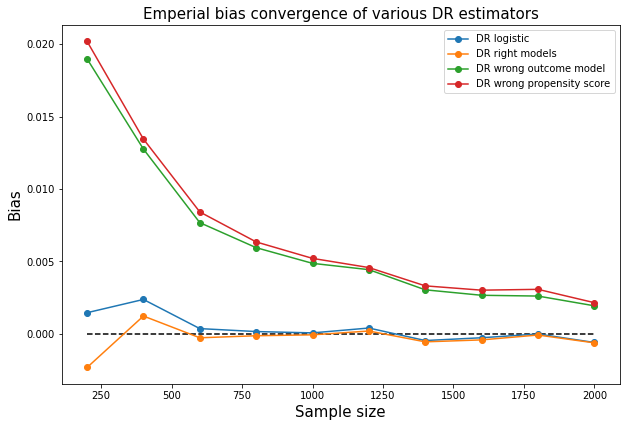
\includegraphics[width = 0.8\columnwidth]{figures/biaspara.png}
    \caption{Simulation results of bias for the various DR estimator specifications}
    \label{figbiaspara}
\end{figure}
\begin{figure}[h!]
    \centering
    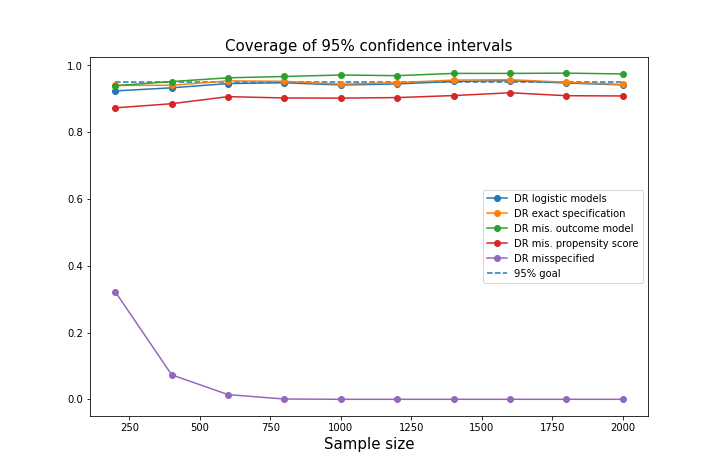
\includegraphics[width = 0.8\columnwidth]{figures/CIpara.png}
    \caption{Simulation results of 95\% confidence intervals coverage for the various DR estimator specifications}
    \label{figCIpara}
\end{figure}
\begin{figure}[h!]
    \centering
    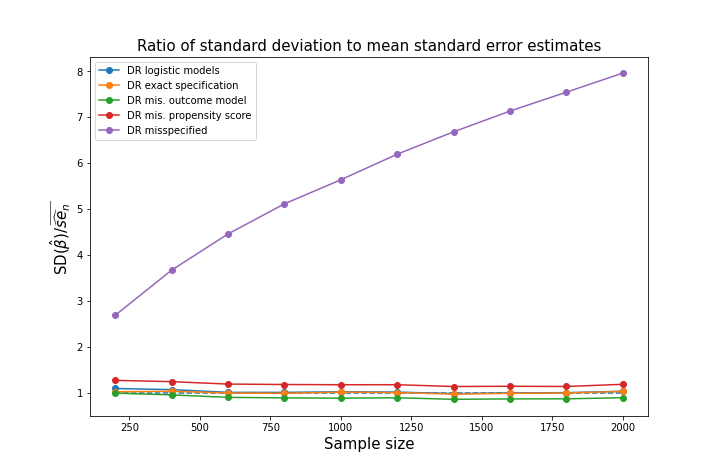
\includegraphics[width = 0.8\columnwidth]{figures/SEpara.png}
    \caption{Accuracy of \citet{lunceford_davidian} SE estimation for the various DR estimator specifications}
    \label{figSEpara}
\end{figure}

Although these results suggest that the parametric methods for setting the nuisance parameters is a good way of specifying these models, as shown by the consistency of the estimates, in reality we were only able to set the models correctly because we knew the distribution of the data generative method, and therefore the fact that there was an interactive term between $W_1,W_2$ in the logistic regression model. Had we been given this data set without any information on how it was generated, it would have been a lot more time-consuming to find the correct specification of at least one nuisance parameter. This is where the practicality of ensemble learners from Machine Learning tools seem to be a more efficient way of setting these models, which we will cover in the next section. Nevertheless, a important advantage of parametric DR estimation is the user-friendly aspect, as we have mentioned previously that logistic or linear regressions models are easy fitting methods to start with.

\section{Machine Learning approaches to optimise the DR estimator}

CURRENTLY A DRAFT - NO NEED FOR FEEDBACK

Parametric models are more certainty but mostly produce biased estimate, but we can apply the central limit theorem and the law of large numbers for convenient asymptotic normality and confidence intervals (CI).

But convenience is over weighed by defectiveness under model misspecification as we mentioned in the previous section, so the probability of the CI containing the true mean converges to 0 \citep{diaz}


Can use machine learning models to alleviate this bias.

Data adaptive methods: random forests, kernel regression, outcome weighed learning, Q-learning, ensemble learners. These methods may not have quantifyable theoretical guarantees though.

\subsection{Using Random Forests}








%% bibliography
\clearpage
\bibliographystyle{unsrtnat}
\bibliography{bibliography}


\end{document}
